\section{Lighting}
\subsection{Preface}
One of the most important factors that make a scene realistic is how the light interacts with the objects in it.
Through time, rendering techniques progressed from various empirical models (e.g. Phong models), that required
tweaking from the artists in order to make results seem more realistic under different lighting setups, to physical based
algorithms (e.g. Microfacet models) that calculate the correct object lighting given the lighting environment and
its material properties. The Physical Based models are based on the laws of physics on how light interacts with
matter depending on a number of environmental variables.

\subsection{Background}
All the physical based rendering models try to solve a simplified version of the rendering equation~\cite{lighting:ref32}.
This equation gives the outgoing light in a particular direction $\omega_o$ from a point $p$ on a surface
and looks like this:

\begin{equation}
\label{eq:rendeq}
L_o(p,\omega_o) = L_e(p, \omega_o) + \int_\Omega f_r(p,\omega_i,\omega_o)L_i(p,\omega_i)n\cdot\omega_i \ d\omega_i
\end{equation}

\noindent Breaking down the equation we get:

\begin{equation}
\underbrace{L_o(p,\omega_o)}_\text{Outgoing Light} = \underbrace{L_e(p, \omega_o)}_\text{Emitted Light} + \underbrace{\int_\Omega f_r(p,\omega_i,\omega_o)L_i(p,\omega_i)n\cdot\omega_i \ d\omega_i}_\text{Integral}
\end{equation}

According to the equation the \textit{outgoing light} in a particular direction from a point on a surface is the sum of the
sum of the \textit{emitted light} from that point and the sum of all the incoming light from all directions in a hemisphere
above the point p (the orientation of the hemisphere is determined by the normal n).

\noindent Breaking down the integral we get:

\begin{equation}
\int_\Omega \underbrace{f_r(p,\omega_i,\omega_o)}_\text{BRDF}\underbrace{L_i(p,\omega_i)}_\text{Incoming Light}\underbrace{n\cdot\omega_i}_\text{Normal Attenuation}\ d\omega_i
\end{equation}

Where BRDF is a function that returns the ratio of the amount of light reflected in a particular direction $\omega_o$, to the
amount received from another direction $\omega_i$ (more details later), incoming light is the light arriving at the point p
from the direction $\omega_i$, and the normal attenuation is an attenuation factor that makes the incoming light at $p$
dependent on the cosine of the angle between the normal $n$ and the incoming light direction $\omega_i$. Note that the
incoming light does not have to come from a light source (direct light), it may have been reflected or refracted from another
point int the scene (indirect light).

\subsection{Diffuse and Specular lighting}
When light hits a surface there are three possible outcomes. Light may be \textbf{absorbed} by the material, light may be
\textbf{transmitted} through to the other side or light may be \textbf{reflected} back.
Reflected light can be divided into two sub-types, specular reflection and diffuse reflection. Specular reflection reflects
all light near the same angle, whereas diffuse reflection reflects in a broad range of directions.
The Cook-Torrance model, that is used in the current implementation, also makes this separation by describing the BRDF
function as:

$$f_r = k_d f_{lambert} + k_s f_{cook-torrance}$$

Where $f_{lambert}$ describes the diffuse component, $f_{cook-torrance}$ describes the specular component, $k_d$ is the amount
of incoming radiance that gets diffused and $k_s$ is the amount of light that is specularly reflected. If a given material
exhibits a strong diffusive behaviour it have a high value for $k_d$, while if it behaves more like a mirror it will have high $k_s$.
For the diffuse BRDF has been choosen the Lambert's BRDF that is equal to:

$$f_{lambert} = \frac{c}{\pi}$$

where c is the surface colour. The specular Cook-Torrance BRDF is defined as:

$$f_{cook-torrance} = \frac{DFG}{(4 \omega_o \cdot n)(\omega_i \cdot n)}$$

Where D is the distribution function, F is the fresnel function and G is the geometry function.
These terms exist, as the Cook-Torrance model falls into the category of the \textbf{Microfacet Models} which revolves around the idea
that rough surfaces can be modelled as a collection of small microfacets, each of them is assumed to be a very small perfect mirror,
and their distribution and orientation define how the light is reflected at a large scale.

\subsection{Material properties}
Materials are defined by the following properties:

\begin{enumerate}
    \item Base Color (Albedo), defines the color of diffused light
    \item Roughness, defines how rough is a surface. Rougher surfaces will show wider but dimmer specular reflections, while smoother
        surfaces will show brighter but sharper specular reflections.
    \item Metallic, defines if a material behaves like a dielectric or metal.
    \item Reflectivity, defines the percentage of light a surface reflects. Specifically defines how reflective a surface is when viewed
        head on.
    \item Emissive Color, defines emission light color for emissive materials.
\end{enumerate}

The separation between metallics and dielectrics, also affects the perspective material colors on each light reflection type.
Metallics are assumed to be fully specular materials with base color acting as their specular color and no diffuse color (black).
In the dielectrics category from the other the base color acts as their diffuse color and white as their specular color.
The above choice can be explained as the subsurface scatter effect is deeper on dielectric materials due to their substantially
lower density comparing to metals.

In the following figures we can see the effects of roughness and reflectivity values for each type of material with
roughness increasing from left to right and increasing from bottom to top:

\begin{figure}[h]
    \centering
    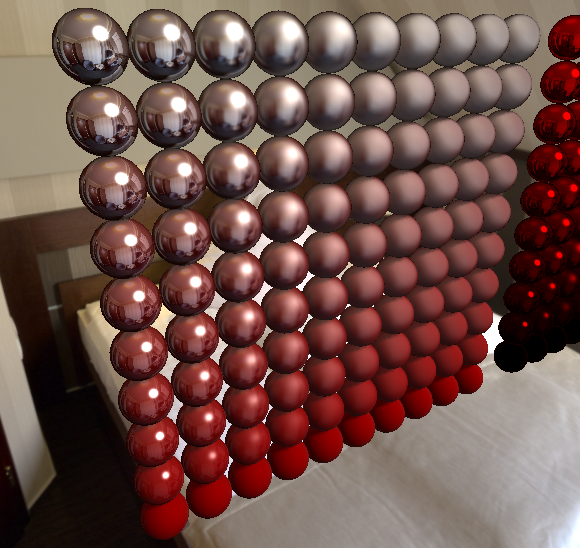
\includegraphics[scale=0.4,clip=true]{./image/pbr_dielectrics.png}
    \caption{Dielectrics}
\label{fig:pbrdielectrics}
\end{figure}

\begin{figure}[h]
    \centering
    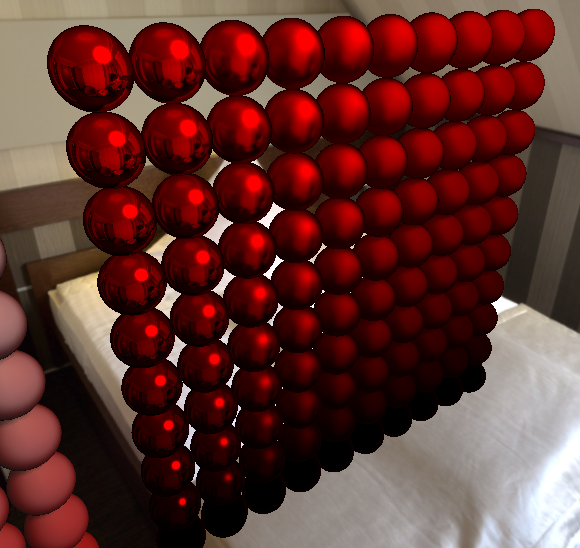
\includegraphics[scale=0.4,clip=true]{./image/pbr_metals.png}
    \caption{Metals}
\label{fig:pbrmetals}
\end{figure}

\subsection{Environmental lighting}
As said in a previous section, light arriving in a point may have been reflected or refracted from another point int the scene.
Offline algorithms may be able to capture that effect but its realtime computation is impossible. So in order to emulate indirect
lighting there is an imminent need for some preprocessing of the surrounding environment of an object.

For this a technique called Image Base Lighting (IBL) can be used. In this technique we first capture the object's environment
as images in a form of a cubemap and then we precalculate the rendering equation integrals treating each pixel in the environment
map as a light source. The results can also be stored in cubemaps that we can then query and use to calculate the environmental
light contribution on a fragment.

\begin{figure}[h]
    \centering
    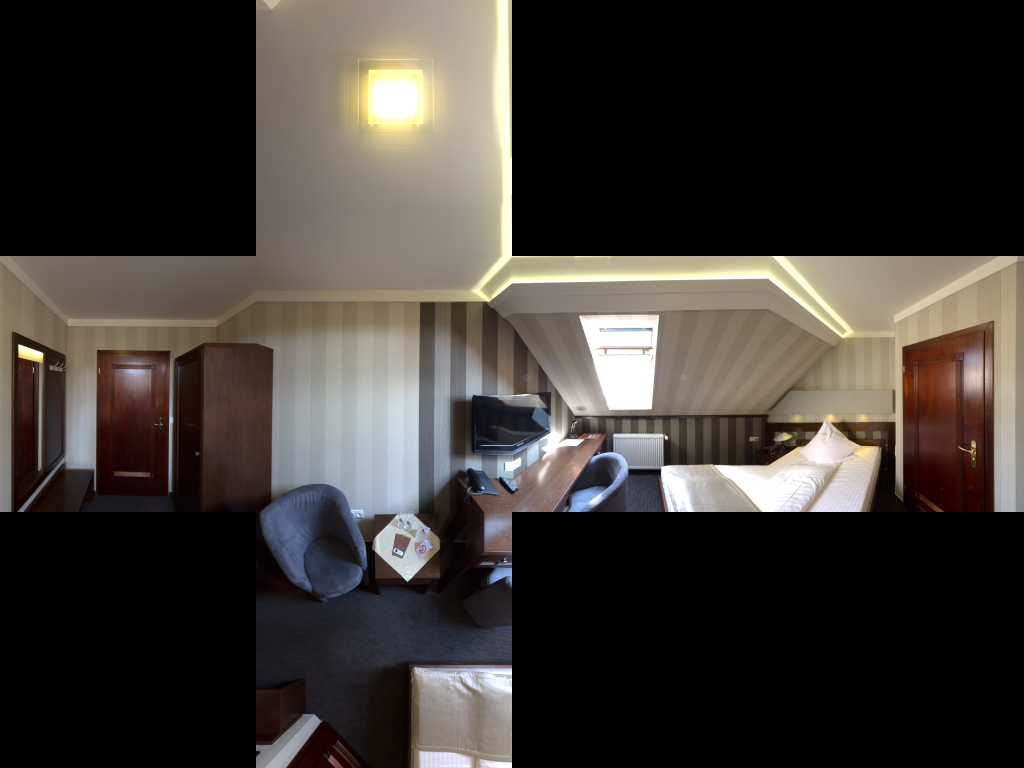
\includegraphics[scale=0.18,clip=true]{./image/envl_ref.png}
    \caption{Reference Environment}
\label{fig:envlref}
\end{figure}

The environmental diffuse light contribution can be captured on something called Irradiance Map. The Irradiance map can be generated
by precalculating Lambert Diffuse BRDF for all the points around an object, and giving the simplicity of the Lambert Diffuse BRDF
function generating it is as simple as applying cosine filter to the reference environment.

\begin{figure}[ht]
    \centering
    
\includegraphics[scale=0.18,clip=true]{./image/envl_irr.png}
    \caption{Irradiance Map}
\label{fig:envlirr}
\end{figure}

The environmental specular light contribution can be captured on the relevant Radiance Map or also called Prefiltered mipmaped
radiance environment map (PMREM). Solving the specular BRDF is more difficult than the diffuse BRDF though, due to the number of
contributing factors. Specifically roughness is the main contributor on the tightness of the specular lobe, so with lower roughness
values a less blurry lookup map is needed, while with the higher roughness values a more blurry map must be used in order to make
the correct specular lobe. For this reason multiple versions of increasing roughness radiance maps are created that are choosen
for their relevant roughness value. These maps can be stored as different mipmaps of the radiance cubemap in order to sample uniformingly.
A function that will choose the correct mipmap level according to an object roughness must be also created, that should be tweaked
for a specific cubemap resolution.

\begin{figure}[ht]
    \centering
    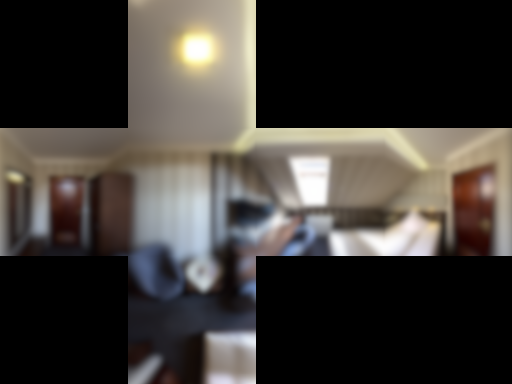
\includegraphics[scale=0.36,clip=true]{./image/envl_rad.png}
    \caption{Radiance Map}
\label{fig:envlrad}
\end{figure}

Note that still, this way only phong lobe shapes are possible to be matched, as the whole microfacet specular
BRDF is not evaluated for the environment, although more advanced approximations also exist\footnote{Split sum approximation is a great
example, where the part of the BRDF not included in the PMREM is calculated as a separate lookup table that can be used to make
specular lobes for the environment lighting that match the direct lighting model}.
